\section{DRRIP}
\label{sec:algorithms:drrip}

\begin{figure}[ht]
    \centering
    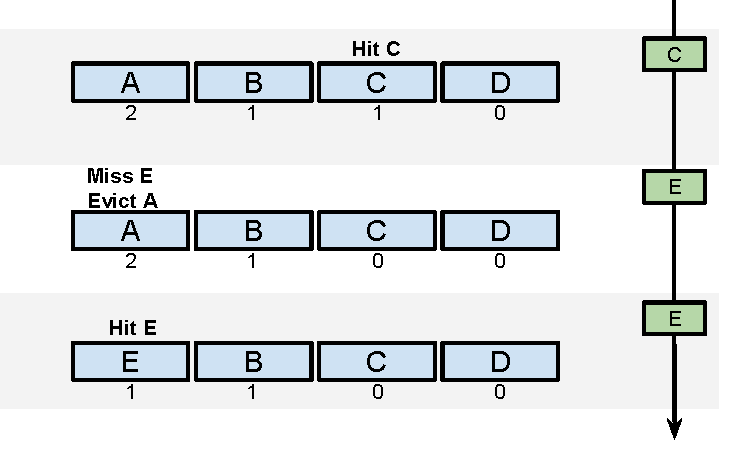
\includegraphics[width=\textwidth]{figures/algorithms/DRRIP}
    \caption{DRRIP managed 4-way cache set (M=2, static insertion).}
    \label{fig:algorithms:drrip_example}
\end{figure}

Dynamic Re-Reference Interval Prediction (DRRIP) was first proposed by A. Jaleel et al.~\cite{Jaleel2010} in 2010.
DRRIP does not utilize the concept of an LRU stack as both LRU and TADIP does.
In DRRIP, each cache block has a number associated with it, called re-reference interval.
The re-reference interval is a measure of the time interval between now and the next time the algorithm expects a block to be re-referenced.
A value between 0 and $2^M - 1$, where M is a configurable parameter, is used to represent the re-reference interval.
The value of 0 indicates a near re-reference interval, the algorithm expects the block to be re-referenced in the near future.
The value $2^M - 1$ indicates a distant re-reference interval while the value of $2^M - 2$ indicates a long re-reference interval.
Multiple blocks may have the same re-reference interval. 
Hence, blocks are not strictly ordered as in the LRU stack.
By setting $M=1$, DRRIP degrades into the Not Recently Used (NRU)~\cite{Microsystems2007} algorithm, which among others is used on the UltraSPARC T2.

The replacement policy of DRRIP is to scan all blocks and evict the first one found with a distance re-reference interval.
If no blocks have a distant re-reference interval the re-reference interval of all blocks are incremented by one and the scan starts over.
This process repeats until the algorithm finds a victim block.
If multiple blocks are potential victims, the algorithm uses the scan order as a tie-breaker.
In the original paper, the authors specify that the leftmost potential block, the one with a lower block index, is the victim.

DRRIP's promotion policy is to decrement the re-reference interval of the accessed block.
By doing this DRRIP utilized access frequency rather than access time to calculate the re-reference interval.
Hence, in order to reach a near re-reference interval a block has to have a high access frequency.
This promotion policy is different compared to LRU and TADIP, where a block will move to the MRU position following a hit, independent of the previous access history.

The insertion policy of DRRIP, like DIP and TADIP, is composed of two different policies and a selection mechanism.
Static RRIP (SRRIP) will always insert new blocks with a long re-reference interval. 
Depending on the state of the cache blocks inserted by SRRIP will therefore potentially have other blocks behind it with a lower re-reference interval.
Binominal RRIP (BRRIP) is analog to BIP in DIP.
BRRIP with either insert new blocks with a distant re-reference interval or, with a small probability, insert like SRRIP with a long re-reference interval.
Like BIP, BRRIP will allow trashing access patterns to keep some of the working set in the cache and hence improve performance over SRRIP.
Selecting between the two insertion policies can be done in using set dueling or ATDs, similar to what was described for TADIP.
The authors use set-dueling in their original paper, and we opt to do this in our implementation as well.

Figure~\ref{fig:algorithms:drrip_example} shows an example cache managed by DRRIP.
In the example, M is set to 2, making the distant re-reference interval 3 and the long re-reference interval 2. 
In addition, we assume static insertion thought the example.
Initially, there are four blocks A, B, C and D with re-reference intervals 2, 1, 1 and 0.
First an access hits the C block, and its value decrements to 0.
Next a miss to block E occurs, and as no block has a re-reference interval of 3 the value of all blocks is incremented by one. 
A then has a value of 3 and is evicted, E in inserted in its place with a value of 2.
Finally, a hit to E occurs causing its value to decrease.